\documentclass{article}
\usepackage[utf8]{inputenc}
\usepackage[margin=3cm]{geometry}
\usepackage{indentfirst}
\usepackage{graphicx}
\usepackage{amsmath}
\graphicspath{ {./images/} }
\setlength{\parindent}{0.75cm} %heh, 0.75

\title{
    \textbf{Programação 3D - Assignment II}
    }
\author{
    \begin{Large}
        \textbf{Grupo 02}
    \end{Large}\\
    Francisco Campaniço 83463\\
    João Rafael 83482\\
    Rodrigo Oliveira 83558
}
\date{Março 2019}

\begin{document}

    \maketitle

    \section*{\textit{Uniform Grid Acceleration}}
        \par
        Para a grelha uniforme usa-se o algoritmo de Amanatides e Woo (1987). Este algoritmo inicializa a grid com um número de células dado por: 
        $$N\_cells_{ax} = \frac{M \cdot dim_{ax}}{(\frac{dim_x \cdot dim_y \cdot dim_z}{N\_obj})^{\frac{1}{3}}} + 1, ax = \{x,y,z\}$$
        $N\_obj$ sendo o número de objetos, $dim$ as dimensões da grelha, e $M$ um fator dado pelo utilizador (usa-se 2 por defeito).
        \par
        Após a criação das células, verifica-se que células é que contém cada objeto. Para isso, calculamos os índices das células correspondentes à \textit{Bounding Box} do objeto:
        $$i_{ax,min/max} = clamp(\frac{(obj\_bb_{ax} - grid\_bb_{ax,min/max})\cdot N\_cells_{ax}}{dim_{ax}},0,N\_cells_{ax} - 1), ax = \{x,y,z\}$$
        e percorremos todos os índices entre $i_{min}$ e $i_{max}$, preenchendo cada célula com ponteiros para os objetos contidos nela.
        \par
        Depois desta inicialização, começam-se a disparar raios sobre a grid, usando o algoritmo acima mencionado de \textit{grid traversal}, que consiste em ver a primeira célula onde o raio acerta, e calcular a trajetória do raio através da grid (ou seja, calcula-se os índices $tnext$, $step$ e $stop$).
        \par
        Finalmente, calcula-se para cada objeto na célula a interseção com o raio, e se não houver nenhuma interseção, ou a interseção tiver uma distância superior à distância até à próxima célula (ou seja, $tnear > tnext$), continua-se o atravessamento para a próxima célula. Este último caso deve-se ao facto de se há interseção mas é mais distante do que a célula atual, não há garantias que na verdade há uma interseção mais próxima, mas numa célula mais distante:
        \begin{center}
            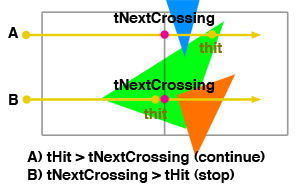
\includegraphics[scale=0.7]{overlap} 
        \end{center}

        \subsection*{Extra: \textit{Mailboxes}}
            \par
            As mailboxes são uma otimização simples. Tem-se um \textit{ID} inteiro único para cada raio. Se esse raio testar a interseção com um objeto e o resultado for falso, adiciona-se ao objeto o \textit{ID}. Se o próximo raio a testar interseção com este objeto for o mesmo (ou seja, \textit{ID} igual), passa-se os cálculos de interseção à frente.
            \par
            Naturalmente, ter um \textit{ID} único não funciona muito bem com paralelização. Como tal, as \textit{mailboxes} são desligadas quando se tem a paralelização ligada.

        \subsection*{Extra: Paralelização}
            \par

        \subsection*{Resultados}
        Foram testadas várias cenas com as diferentes otimizações. O CPU usado foi um Intel i7-8750H com 6 \textit{cores} e 12 \textit{threads}.
        \begin{table}[h]
            \centering
            \begin{tabular}{|l|l|l|l|l|}
                \hline
                Teste                      & Sem Grid & Grid  & Grid + Mailboxes & Grid + Paralelização \\ \hline
                Balls (High)               & 12m14s   & 0m15s & 0m14s            & 1s500ms              \\ \hline
                Mount (Very High)          & 2h21m3s  & 0m32s & 0m29s            & 5s500ms              \\ \hline
                BFBoat (4000 triângulos)   & 14m45s   & 0m15s & 0m12s            & 1s700ms              \\ \hline
                Distant (3 esferas, DoFx32)& 0m29s    & 0m26s & 0m25s            & 5s300ms              \\ \hline
            \end{tabular}
        \end{table}


    \section*{\textit{Anti-Aliasing}}
        \par


    \section*{\textit{Soft Shadows}}
        \subsection*{\textit{Area Light}}
            \par
            Este método baseia-se em simular as luzes como áreas em vez de \textit{pointlights}. Para isto, calculam-se "posições alternativas" para cada luz, que consistem de um deslocamento da posição de cada luz dentro de uma área definida previamente, e com um pouco de \textit{jittering}:
            $$ light\_alternate\_pos = \{x + \frac{p + rand}{samples * area}, y + \frac{q + rand}{samples * area}, z\}, p,q \in \{0, samples - 1\},$$
            $rand$ sendo um valor aleatório entre 0 e 1. Após calcular estas posições, da-se \textit{shuffle} ao vetor que as contém, para que cada pixel \textit{jittered} não teste as sombras com a sua posição correspondente:
            \begin{center}
                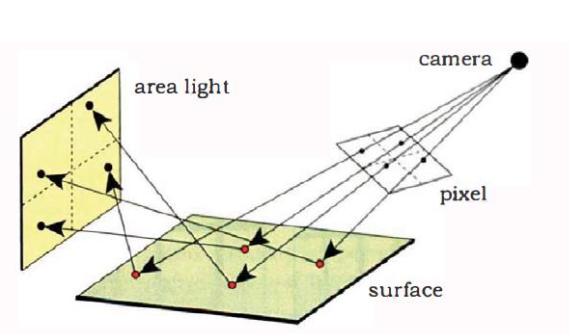
\includegraphics[scale=0.5]{area} 
            \end{center}

        
    \section*{\textit{Depth of Field}}
        \par

    \section*{Extras}  
        \subsection*{Ficheiros PLY}
        \par

        \subsection*{\textit{Glossy Reflections}}  
        \par

\end{document}